\section{积分与极限}
\label{sec:integ-limits}

分析中的许多函数是逐步逼近得到的：级数的部分和、截断区间上的函数、越来越细的平均。若一列可测函数逐点趋于目标函数，我们希望各次积分也趋于目标函数的积分，这样就能用容易计算的近似求出难以直接计算的积分。本节先说明逐点与几乎处处收敛的含义，用一个尖峰例子说明交换不能无条件进行；再依次研究递增逼近、非负函数列的下极限估计，以及由同一个可积函数控制的函数列。收敛方式的系统比较以及一致可积性，留到第~\ref{chap:normed-spaces}章。

\subsection{逐点逼近与积分极限}
\label{sec:integ-pointwise}

\paragraph{逐点收敛与几乎处处收敛}
固定一个输入点$x$，函数列$f_1,f_2,\dots$在这一点的取值是一列数$f_1(x),f_2(x),\dots$。若对每个$x\in X$，这列数都收敛到$f(x)$，称$f_n$\term{逐点收敛}（pointwise convergence）到$f$。积分看不见零测集，所以只需要求收敛在零测集之外成立：若存在零测集$N$，使$f_n(x)\to f(x)$对每个$x\notin N$成立，称$f_n$\term{几乎处处收敛}（almost everywhere convergence）到$f$。

几乎处处的极限只确定到零测集。若$f_n$几乎处处收敛到$f$与$g$，两个例外集之并仍是零测集，在它之外$f=g$，所以$f=g$几乎处处成立。极限函数的可测性也要留意：收敛点集$\{x:\limsup_nf_n(x)=\liminf_nf_n(x)\}$可测，在其上取$\limsup_nf_n$、其外取$0$，就得到一个可测的极限代表；在完备测度空间中，任何几乎处处等于它的函数都可测。下面谈到几乎处处收敛的极限时，总指这样一个可测代表。

\paragraph{积分不随逐点极限收敛的例子}
在$[0,1]$上取
\[
 f_n(x)=n\mathbf 1_{(0,1/n)}(x),\qquad n\geq1.
\]
对$x=0$，每个$f_n(0)=0$；对$x>0$，当$n>1/x$时$x\notin(0,1/n)$，$f_n(x)=0$。所以$f_n$逐点收敛到$0$。但每个$f_n$是高为$n$、宽为$1/n$的矩形，$\int f_n=1$，于是
\[
 \lim_{n\to\infty}\int_{[0,1]}f_n\,\mathrm d\lambda=1\neq0=\int_{[0,1]}\lim_{n\to\infty}f_n\,\mathrm d\lambda .
\]
质量没有消失，而是挤进了越来越窄的区间：每一点最终都看不到尖峰，尖峰的面积却始终是$1$。这说明积分与极限的交换需要条件。下面三小节给出三种条件：函数列递增，函数列非负（只得到单向估计），以及函数列被一个可积函数共同控制。

\subsection{单调收敛}
\label{sec:integ-monotone-convergence}

\paragraph{单调收敛定理}
尖峰例子中的函数列不单调：$f_n$在$(0,1/n)$上增大，在别处变为零。若函数列递增，质量只会不断加入，不会挤走，积分就能与极限交换。引理~\ref{lem:integ-increasing-simple}对递增的简单函数列证明了这一点，同样的论证对一般的递增可测函数列成立。

\begin{theorem}[单调收敛定理]
\label{thm:integ-monotone-convergence}
设$f_n:X\to[0,+\infty]$可测，$f_1\leq f_2\leq\cdots$几乎处处成立，$f=\lim_nf_n$几乎处处成立。则
\[
 \int_Xf\,\mathrm d\mu=\lim_{n\to\infty}\int_Xf_n\,\mathrm d\mu,
\]
两边在$[0,+\infty]$中相等。
\end{theorem}

\begin{proof}
把可数个例外零测集合并为$N$，在$N$上把$f$与全部$f_n$改为$0$，积分都不变，所以不妨设单调性与收敛处处成立。由单调性，$\int f_n$递增且不超过$\int f$，极限存在且不超过$\int f$。

反方向，任取简单函数$0\leq s\leq f$与$c\in(0,1)$，令$E_n=\{f_n\geq cs\}$。它们可测且递增；与引理~\ref{lem:integ-increasing-simple}的证明相同，$s(x)>0$时$f(x)>cs(x)$，所以$\bigcup_nE_n=X$。于是$\int f_n\geq c\int s\mathbf 1_{E_n}\to c\int s$。令$c\uparrow1$，再对$s$取上确界，得$\lim_n\int f_n\geq\int f$。
\end{proof}

积分值允许为$+\infty$：若$\int f=+\infty$，定理说$\int f_n\to+\infty$。非负性也不能省去，否则会遇到$\int f_1=-\infty$这样无法向上逼近的起点；只要$f_1$可积，对$f_n-f_1$应用定理即可处理取负值的递增列。

\paragraph{非负级数与可数区域}
递增列最常见的来源是非负项的部分和与逐步扩大的区域。设$g_k\geq0$可测，部分和$\sum_{k\leq n}g_k$递增到$\sum_kg_k$，由单调收敛定理与有限可加性，
\begin{equation}
 \int\sum_{k=1}^\infty g_k\,\mathrm d\mu=\sum_{k=1}^\infty\int g_k\,\mathrm d\mu .
 \label{eq:integ-series-termwise}
\end{equation}
非负函数项级数总可以逐项积分，两边允许为$+\infty$。取$g_k=f\mathbf 1_{A_k}$，其中$A_k$两两不交，就得到第~\ref{sec:integ-domain-additivity}小节预告的可数区域分解$\int_{\bigcup_kA_k}f=\sum_k\int_{A_k}f$；所以对非负可测的$f$，$A\mapsto\int_Af\,\mathrm d\mu$是测度。

两个计算说明式~\eqref{eq:integ-series-termwise}的用法。在$\mathbb N$上取计数测度，非负函数$f=\sum_nf(n)\mathbf 1_{\{n\}}$，逐项积分得$\int f=\sum_nf(n)$：离散空间上的非负积分就是级数求和。在$[0,1)$上，$-\log(1-x)=\sum_{n\geq1}x^n/n$各项非负，逐项积分并用定理~\ref{thm:integ-riemann-lebesgue}计算多项式的积分，得
\[
 \int_{[0,1)}-\log(1-x)\,\mathrm dx=\sum_{n\geq1}\frac1{n(n+1)}=\sum_{n\geq1}\Bigl(\frac1n-\frac1{n+1}\Bigr)=1 .
\]

\paragraph{反常积分定理的证明}
现在补上第~\ref{sec:integ-improper}小节的依据。

\begin{proof}[定理~\ref{thm:integ-improper}的证明]
取$b_n\uparrow\beta$。由定理~\ref{thm:integ-riemann-lebesgue}，每个$f\mathbf 1_{[a,b_n]}$关于$\mathcal L$可测，它们逐点收敛到$f\mathbf 1_I$，所以$f$在$I$上可测。

第1条：$f\geq0$时$f\mathbf 1_{[a,b_n]}$递增到$f\mathbf 1_I$，单调收敛定理与定理~\ref{thm:integ-riemann-lebesgue}给出$\int_If\,\mathrm d\lambda=\lim_n\int_a^{b_n}f\,\mathrm dx$。由于$b\mapsto\int_a^bf$递增，沿任意$b_n\uparrow\beta$的极限都等于$b\uparrow\beta$时的极限。

第2条：$\lvert f\rvert$在每个$[a,b]$上黎曼可积（它的振幅不超过$f$的振幅），由第1条$\int_I\lvert f\rvert\,\mathrm d\lambda=\lim_{b\uparrow\beta}\int_a^b\lvert f\rvert$，可积性的等价随之成立。可积时$f^\pm=\frac12(\lvert f\rvert\pm f)$也在每个$[a,b]$上黎曼可积，由第1条$\int_If^\pm\,\mathrm d\lambda=\lim_b\int_a^bf^\pm$，两个极限都有限，相减即得。
\end{proof}

\subsection{Fatou估计}
\label{sec:integ-fatou}

\paragraph{下极限的积分}
对不单调的非负函数列，尖峰例子说明等式可以失败。但失败只有一个方向：极限函数的积分不会\emph{超过}积分的极限，因为非负函数的质量只能在极限中丢失，不能凭空产生。把不单调的列换成它的尾部下确界，就得到一个递增列，可以用单调收敛定理。

\begin{theorem}[Fatou引理]
\label{thm:integ-fatou}
设$f_n:X\to[0,+\infty]$可测。则
\[
 \int_X\liminf_{n\to\infty}f_n\,\mathrm d\mu\leq\liminf_{n\to\infty}\int_Xf_n\,\mathrm d\mu .
\]
\end{theorem}

\begin{proof}
令$g_n=\inf_{k\geq n}f_k$。它们是非负可测函数，关于$n$递增，极限为$\liminf_nf_n$。由单调收敛定理，$\int\liminf_nf_n=\lim_n\int g_n$。又对每个$k\geq n$有$g_n\leq f_k$，所以$\int g_n\leq\inf_{k\geq n}\int f_k$。令$n\to\infty$，右边趋于$\liminf_n\int f_n$。
\end{proof}

\paragraph{严格不等与单向性}
在尖峰例子中，$\liminf_nf_n=0$，左边为$0$，右边为$1$，不等式严格成立。所以Fatou引理一般只给出单向估计：当我们知道$\int f_n$有界时，它保证极限函数可积，并给出积分的上界，却不给出积分的值。

非负性不能省去。把尖峰换成$-f_n=-n\mathbf 1_{(0,1/n)}$，下极限仍为$0$，左边为$0$，右边为$-1$，不等式反向。这说明Fatou引理依赖的是“质量只会丢失”这一非负性质。对取正负值的函数列，若有一个可积函数从下方控制它，可以先加上这个函数再用Fatou引理，下一小节正是这样做的。

\subsection{支配收敛}
\label{sec:integ-dominated-convergence}

\paragraph{支配收敛定理}
尖峰的质量能够逃逸，是因为$f_n$的高度没有共同的可积上界。若所有$f_n$都被同一个可积函数压住，质量就无处可逃：它不能挤进越来越窄的区间无限升高，也不能向无穷远处流走。

\begin{theorem}[支配收敛定理]
\label{thm:integ-dominated-convergence}
设$f_n$是实值或复值可测函数，$f_n\to f$几乎处处成立，并且存在可积函数$g\geq0$，使对每个$n$都有$\lvert f_n\rvert\leq g$几乎处处成立。则$f$可积，
\[
 \lim_{n\to\infty}\int_X\lvert f_n-f\rvert\,\mathrm d\mu=0,\qquad \lim_{n\to\infty}\int_Xf_n\,\mathrm d\mu=\int_Xf\,\mathrm d\mu .
\]
\end{theorem}

\begin{proof}
合并可数个例外零测集，不妨设收敛与控制处处成立。先设$f_n$实值。由$\lvert f_n\rvert\leq g$取极限得$\lvert f\rvert\leq g$，所以$f$可积。令$h_n=2g-\lvert f_n-f\rvert$，由$\lvert f_n-f\rvert\leq\lvert f_n\rvert+\lvert f\rvert\leq2g$知$h_n\geq0$，且$h_n\to2g$。由Fatou引理，
\[
 \int2g\leq\liminf_n\int\bigl(2g-\lvert f_n-f\rvert\bigr)=\int2g-\limsup_n\int\lvert f_n-f\rvert,
\]
其中等号用了线性性，$\int2g$有限，可以从两边消去，得$\limsup_n\int\lvert f_n-f\rvert\leq0$。再由绝对值估计$\lvert\int f_n-\int f\rvert\leq\int\lvert f_n-f\rvert\to0$。

复值情形，记$f_n=u_n+\mathrm iv_n$。$\lvert u_n\rvert,\lvert v_n\rvert\leq\lvert f_n\rvert\leq g$，实部与虚部分别几乎处处收敛，由实值情形分别交换极限与积分；误差$\int\lvert f_n-f\rvert\leq\int\lvert u_n-u\rvert+\int\lvert v_n-v\rvert\to0$。
\end{proof}

结论$\int\lvert f_n-f\rvert\to0$比积分值收敛更强：它说的是近似函数整体上接近目标，而不仅是总量接近。由上一节的误差控制，它对每个可测子集$A$同时给出$\lvert\int_Af_n-\int_Af\rvert\leq\int\lvert f_n-f\rvert\to0$。

\paragraph{共同上界的作用}
图~\ref{fig:integ-dominating-envelope}对照了一个可控与一个不可控的例子。在$[0,1]$上$f_n(x)=x^n$逐点收敛到$\mathbf 1_{\{1\}}$，几乎处处为零，所有$f_n$都被常数$1$控制，常数在$[0,1]$上可积，所以$\int x^n=1/(n+1)\to0$，与支配收敛一致。

尖峰列$f_n=n\mathbf 1_{(0,1/n)}$没有可积的控制函数。任何控制函数都不小于上包络$h=\sup_nf_n$，而$h$在$[\frac1{n+1},\frac1n)$上等于$n$，于是$h(x)\geq1/x-1$，后者在$(0,1)$上积分为$+\infty$。这正是积分极限失败的原因：共同上界缺失时，质量可以集中到越来越小的集合上。

\begin{figure}[!htbp]
 \centering
 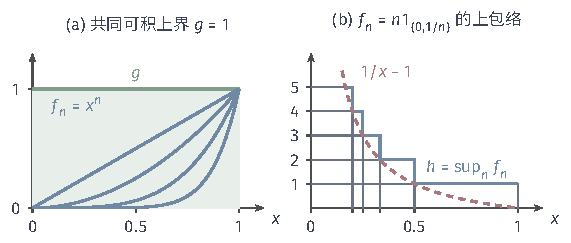
\includegraphics[width=96.633mm]{figures/02-abstract-mathematics/01-metric-and-measure/tikz/c3-dominating-envelope/figure.pdf}
 \caption{控制函数与上包络。(a)$[0,1]$上$f_n=x^n$（$n=1,2,4,8$）都位于可积函数$g=1$之下，积分$1/(n+1)\to0$。(b)$f_n=n\mathbf 1_{(0,1/n)}$（灰色，$n=1,\dots,5$）积分恒为$1$；上包络$h=\sup_nf_n$（蓝色阶梯）在$[\frac1{n+1},\frac1n)$上等于$n$，不小于$1/x-1$（红色虚线），后者在$(0,1)$上积分为$+\infty$，所以不存在可积的控制函数。}
 \label{fig:integ-dominating-envelope}
\end{figure}

支配条件是充分而非必要的：有些函数列没有可积的共同上界，积分仍然收敛。刻画积分收敛的确切条件需要一致可积性，它与依测度收敛等收敛方式一起在第~\ref{chap:normed-spaces}章讨论。在有限测度空间上，最常用的特例是：一致有界且几乎处处收敛的函数列，以常数为控制函数，积分可以与极限交换。
